%!TEX root = ../thesis.tex
%*******************************************************************************
%*********************************** First Chapter *****************************
%*******************************************************************************

\chapter{Introduction}\label{chap:intro}  %Title of the First Chapter

\ifpdf
    \graphicspath{{Chapter1/Figs/Raster/}{Chapter1/Figs/PDF/}{Chapter1/Figs/}}
\else
    \graphicspath{{Chapter1/Figs/Vector/}{Chapter1/Figs/}}
\fi


%********************************** %First Section  **************************************
\section{Motivation} %Section - 1.1 

Animal welfare is an important concern for business and society, with an estimated 70 billion animals currently living under human care~\cite{FAOSTAT}. Across multiple industries, monitoring and assessing animal health is achieved by measuring individuals' body shape and movement. These measurements should be taken without interfering with the animal's normal activity, and are needed around the clock, under a variety of lighting and weather conditions, perhaps at long range (e.g.\ in farm fields or wildlife parks). 

Of course, employing humans to monitor large animal populations is costly and can lead to data bias. For example, prey animals such as rodents are known to alter their behaviour in the presense of perceived predators. To overcome this, a number of animal monitoring systems have been designed, especially for use in clinical work. Many systems are `invasive', meaning they require animals to undergo a surgical operation (generally to implant a tracking chip) before monitoring can take place. Although these systems can offer detailed biometric data (such as blood pressure, ECG etc.), the implantation procedure is costly and can cause stress to the animals, leading to welfare concerns and complex behavioural effects. 

Since even crudest system can ensure some basic health standard (e.g.\ to check that \emph{some} activity occurs over a given time period), some systems further attempt to monitor the animals' physical activity. 

To overcome this, a number of non-invasive systems are available. The most basic of these can still be surprisingly effective, for example checking that \emph{some} motion has occured during a given time period can offer an important health standard. More advanced systems can also estimate energy and inquisitiveness levels of the target animals by analysing motion patterns over time. Most systems achieve this by either placing floor-level pressure pads~\cite{zammit2010reliability}, or by installing an overhead camera which performs simple visual blob detection via colour thresholding~\cite{tort2006simple}, \cite{rodriquez2017toxtrac}. One such open source system instructs the user to set a colour tolerance that masks all non-animal pixels and provide expected maximum and minimum animal sizes (in pixels) to help eliminate noise. While this is effective at tracking multiple animals with distinctive colour when placed in an arena with a solid, fixed background, it does not work well in many scenarios, e.g.\ outdoors. The presence of changing light levels, casting of shadows across tracking targets or moving backgrounds (e.g.\ foliage) make such thresholds ineffective. Further, this system's ability to distinguish between multiple tracked subjects is hindered when animals cross one another, as two individual blobs temporarily become one, and from then on are difficult to resolve.

Some work has been done in automatic behavioural scoring for rodents, in which up to ten predefined behaviours can be visually recognized. These approaches typically employ machine learning algorithms, which are taught to recognize behaviours present in a video stream by analyzing a large set of pre-collected examples. For `normal' behaviours (e.g. drinking, eating etc.) this can be a viable approach and by analyzing the changing frequency of such behaviours can indeed offer insights into underlying conditions. However, these systems cannot be readily extended to handle more serious conditions (e.g. animals experiencing a seizure), due to the ethical concerns associated with collecting sufficient examples for training. 

In addition, many 
Of course, even if a behaviour detection system were built for a range of animal species this 

% TODO: Explain why these are of limited use for robust 3D tracking.
% -> Cannot collect behavioural training data for adverse effects
% -> Weight estimation
% -> Platform for future machine learning tools

% Say that we want it to be cheap!

Unfortunately, all these approaches suffer as they fail to reconstruct a full 3D mesh.

% Between farmyards, research facilities, zoos, animal rescue centres, veterinary centres and sporting centres, over 100 billion animals are currently living under human care \cite{FAOSTAT}. For ethical and financial reasons, these industries often rely on the health and wellbeing of their animal populations and there can be dramatic consequences afforded to organizations deemed to fall short. Pressure groups have been particularly critical of zoos and entertainment industries for their inability to identify and treat behaviour disorders. In some cases, this has necessitated expensive re-homing procedures for animals with late-identified psychosis (commonly stereotypy)~\cite{Guardian-Elephant}. Worse still, some have suggested a link between animal health and welfare and loss of human life~\cite{SWOH-Tilikum}.

% This project is funded by GlaxoSmithKline (GSK), a global pharmaceutical company based in the United Kingdom. In order to sell medications for use in humans, GSK and similar companies have a legal obligation to run controlled clinical trials on animal subjects. For reasons of ethics and promotion of good science, the emphasis on animal welfare is paramount. Strict measures are imposed to minimize any potential animal suffering and to maximize useful data output during the study period. By refining existing methods of behaviour analysis, GSK aim to further reduce the numbers of animals required for testing and support robust conclusions about candidate medications at earlier opportunities. Progress here should assist scientists in identifying medicinal side-effects and promote early attrition of the clinical trial, that is, the process of preventing an unsuitable drug compound from progressing in the R\&D pipeline and thereby reducing any further unnecessary expenditure.

% Within sectors concerned with animal husbandry, there is growing support for a system able to continuously monitor captive animals throughout their entire lifetimes. Due to staff working hours and typically large population sizes, it can be impractical for zookeepers or lab technicians to keep continuous watch over all animals under their care at all times. These issues are particularly acute for nocturnal animals in which symptoms may only become apparent during the night, and `prey' animals that have evolved to deliberately hide pain from perceived predators as a defence mechanism. Rats and mice, the two most common species used in animal research, pose both of these challenges.

%********************************** %Second Section  *************************************
\section{Approach} %Section - 1.2

This thesis focuses on developing methods for recovering a 3D model of an animal oa tracking system to enable recovery of a per-frame 3D animal reconstruction from an image or video stream. 

The system should apply to a wide range of animal species without significant customization. Success in this endeavour would enable real-time changes of a known skeletal structure to be programmatically analysed to completely model an animal’s movements. These behaviour patterns could then be interpreted to form a profile for each animal in a batch, taking into account expected norms for their species as well as their individual personality traits. When animals are first brought into a facility, they are given some time to acclimatize to their new surroundings before a clinical study begins. The application could make use of this period to refine behaviour models to their particular characteristics without being influenced by external factors. The system would then begin monitoring the population, storing detailed analytics and reacting to any deviations to an animal’s unique behaviour profile. As a simple example, should a typically lively and sociable dog suddenly begin exhibiting signs of withdrawal from the group, this would indicate a cause for concern and be stored in that animal’s ‘virtual log book’. In some cases, an animal may begin to exhibit signals that demand immediate attention, such as a dramatic and sudden energy drop that may indicate pain. The application could handle such events by sending an SMS text message to an on-call veterinary professional, to alert them of the specific problem and thereby enable a rapid response. These real-time diagnostics could then be aggregated and displayed on a dashboard screen, visible to all laboratory technicians. A concept drawing is shown in Figure \ref{fig:wellness_dashboard}.

\subsection{Problem definition}
    A major challenge of this work is to develop and adapt methods for resolving the inherent ambiguity associated with recovering a 3D model from 2D input data. This challenge can be overcome by augmenting the input video sequence (Figure \ref{fig:arap_input}) with strong prior knowledge about the target species class (e.g.\ quadruped body measurements). This prior knowledge can be divided into two components: a \emph{shape} prior that enforces topological (e.g.\ order of body parts) and measurement constraints (e.g.\ length of limbs), and a \emph{pose} prior that defines likely limb configurations and can be used to rule out those which are anatomically impossible.

    \begin{figure}[H]
        \centering
        \begin{subfigure}{0.33\textwidth}
        \centering
            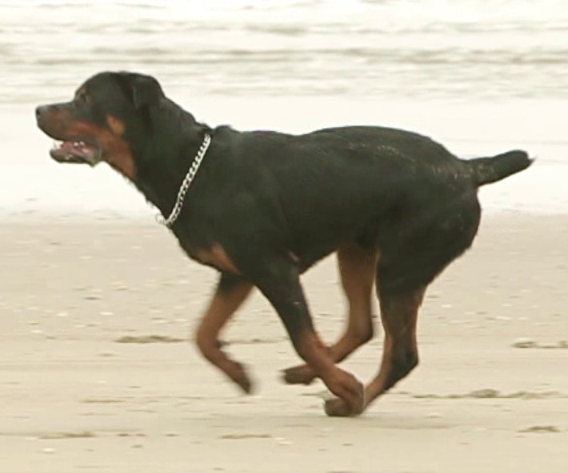
\includegraphics[width=1\linewidth]{input/66}
        \end{subfigure}%
        \begin{subfigure}{0.33\textwidth}
        \centering
            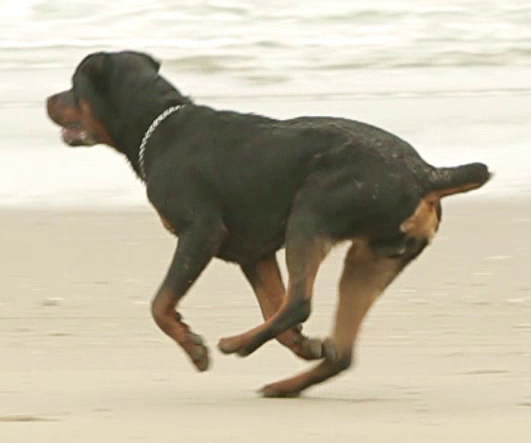
\includegraphics[width=1\linewidth]{input/167}
        \end{subfigure}%
        \begin{subfigure}{0.33\textwidth}
        \centering
            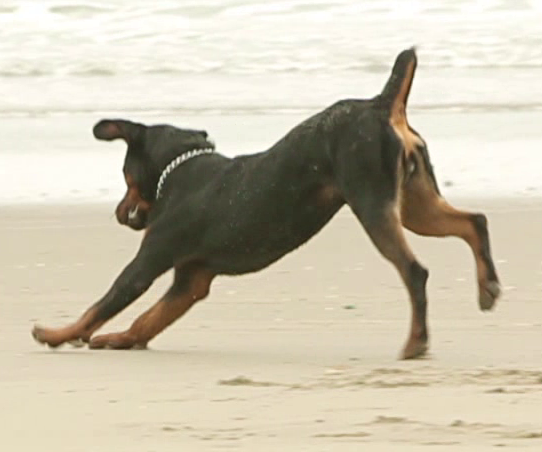
\includegraphics[width=1\linewidth]{input/208}
        \end{subfigure}%
        \caption{An example input video sequence.}
        \label{fig:arap_input}
    \end{figure}

    An example output showing the recovery of a 3D model from an input 2D monocular video is shown in Figure \ref{fig:intro_arap_output}:
    
    \begin{figure}[H]
        \centering
        \begin{subfigure}{1\textwidth}
        \centering
            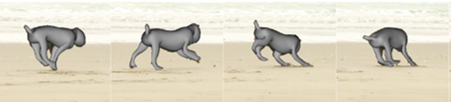
\includegraphics[width=1\linewidth]{input/arapsfm_output}
        \end{subfigure}%
        \caption{Sample output printed from Deformable Mesh Animation~\cite{arap_stebbing}.}
        \label{fig:intro_arap_output}
    \end{figure}

    
    A distinction should be made between two common tracking techniques: (1) discriminative body part recognizers and joint position predictors, and (2) 3D reconstructions via generative model fitting. Discriminative predictors have become the dominant paradigm in human body tracking to facilitate common use-cases, such as gesture detection or controllerless gameplay. However, recovering 3D models from human subjects is a growing field. Applications are found in fashion to faciliate online `try-ons' for virtual clothing~\cite{lin2014digital}, in animation and visual effects to generate virtual characters from live actor performances~\cite{laine2017production}, and in healthcare for tracking patients' body weight over time~\cite{velardo2010weight}. It is hypothesized that recovering a full 3D animal reconstruction is necessary to enable the intended diagnostic purposes of this animal work. In particular, returning only joint positions or body parts may be insufficient to estimate animal weight. If this can be realized, identifying behavioural changes from the reconstruction is expected to be a relatively straightforward machine learning problem. 

    A typical method for recovering 3D structure from tracking targets is using a \emph{model fitting} approach, in which a 3D object representative of the target class is adapted to recreate the performance of the target. This method involves: (1) parameterizing a representative 3D \emph{template mesh} with terms that represent shape and pose attributes and (2) defining an optimizer to adapt to these per-frame parameter settings to an input video sequence. An example of a template mesh is shown in Figure~\ref{fig:arap_template}.
    
    \begin{figure}[H] % Example image
        \center{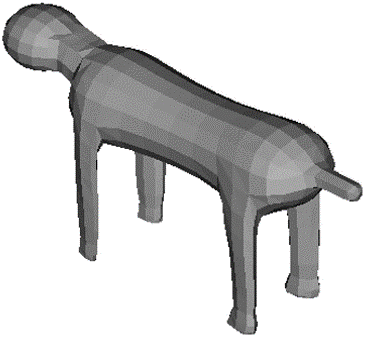
\includegraphics[width=0.2\linewidth]{template_mesh}}
        \caption{An example prior, in this case a template mesh.}
        \label{fig:arap_template}
    \end{figure}

    Shape attributes capture variation between different members of the target class and remain constant for a particular individual. For example, shape parameters may be adapted to vary a model's height and weight. However, pose attributes generally capture limb positions and joint angles, and therefore tend to vary considerably during a capture sequence. Figure~\ref{fig:black_shape} highlights the difference by keeping pose parameters fixed while shape attributes are varied between the three models~\cite{Streuber:SIGGRAPH:2016}.

    \begin{figure}[H] % Example image
        \center{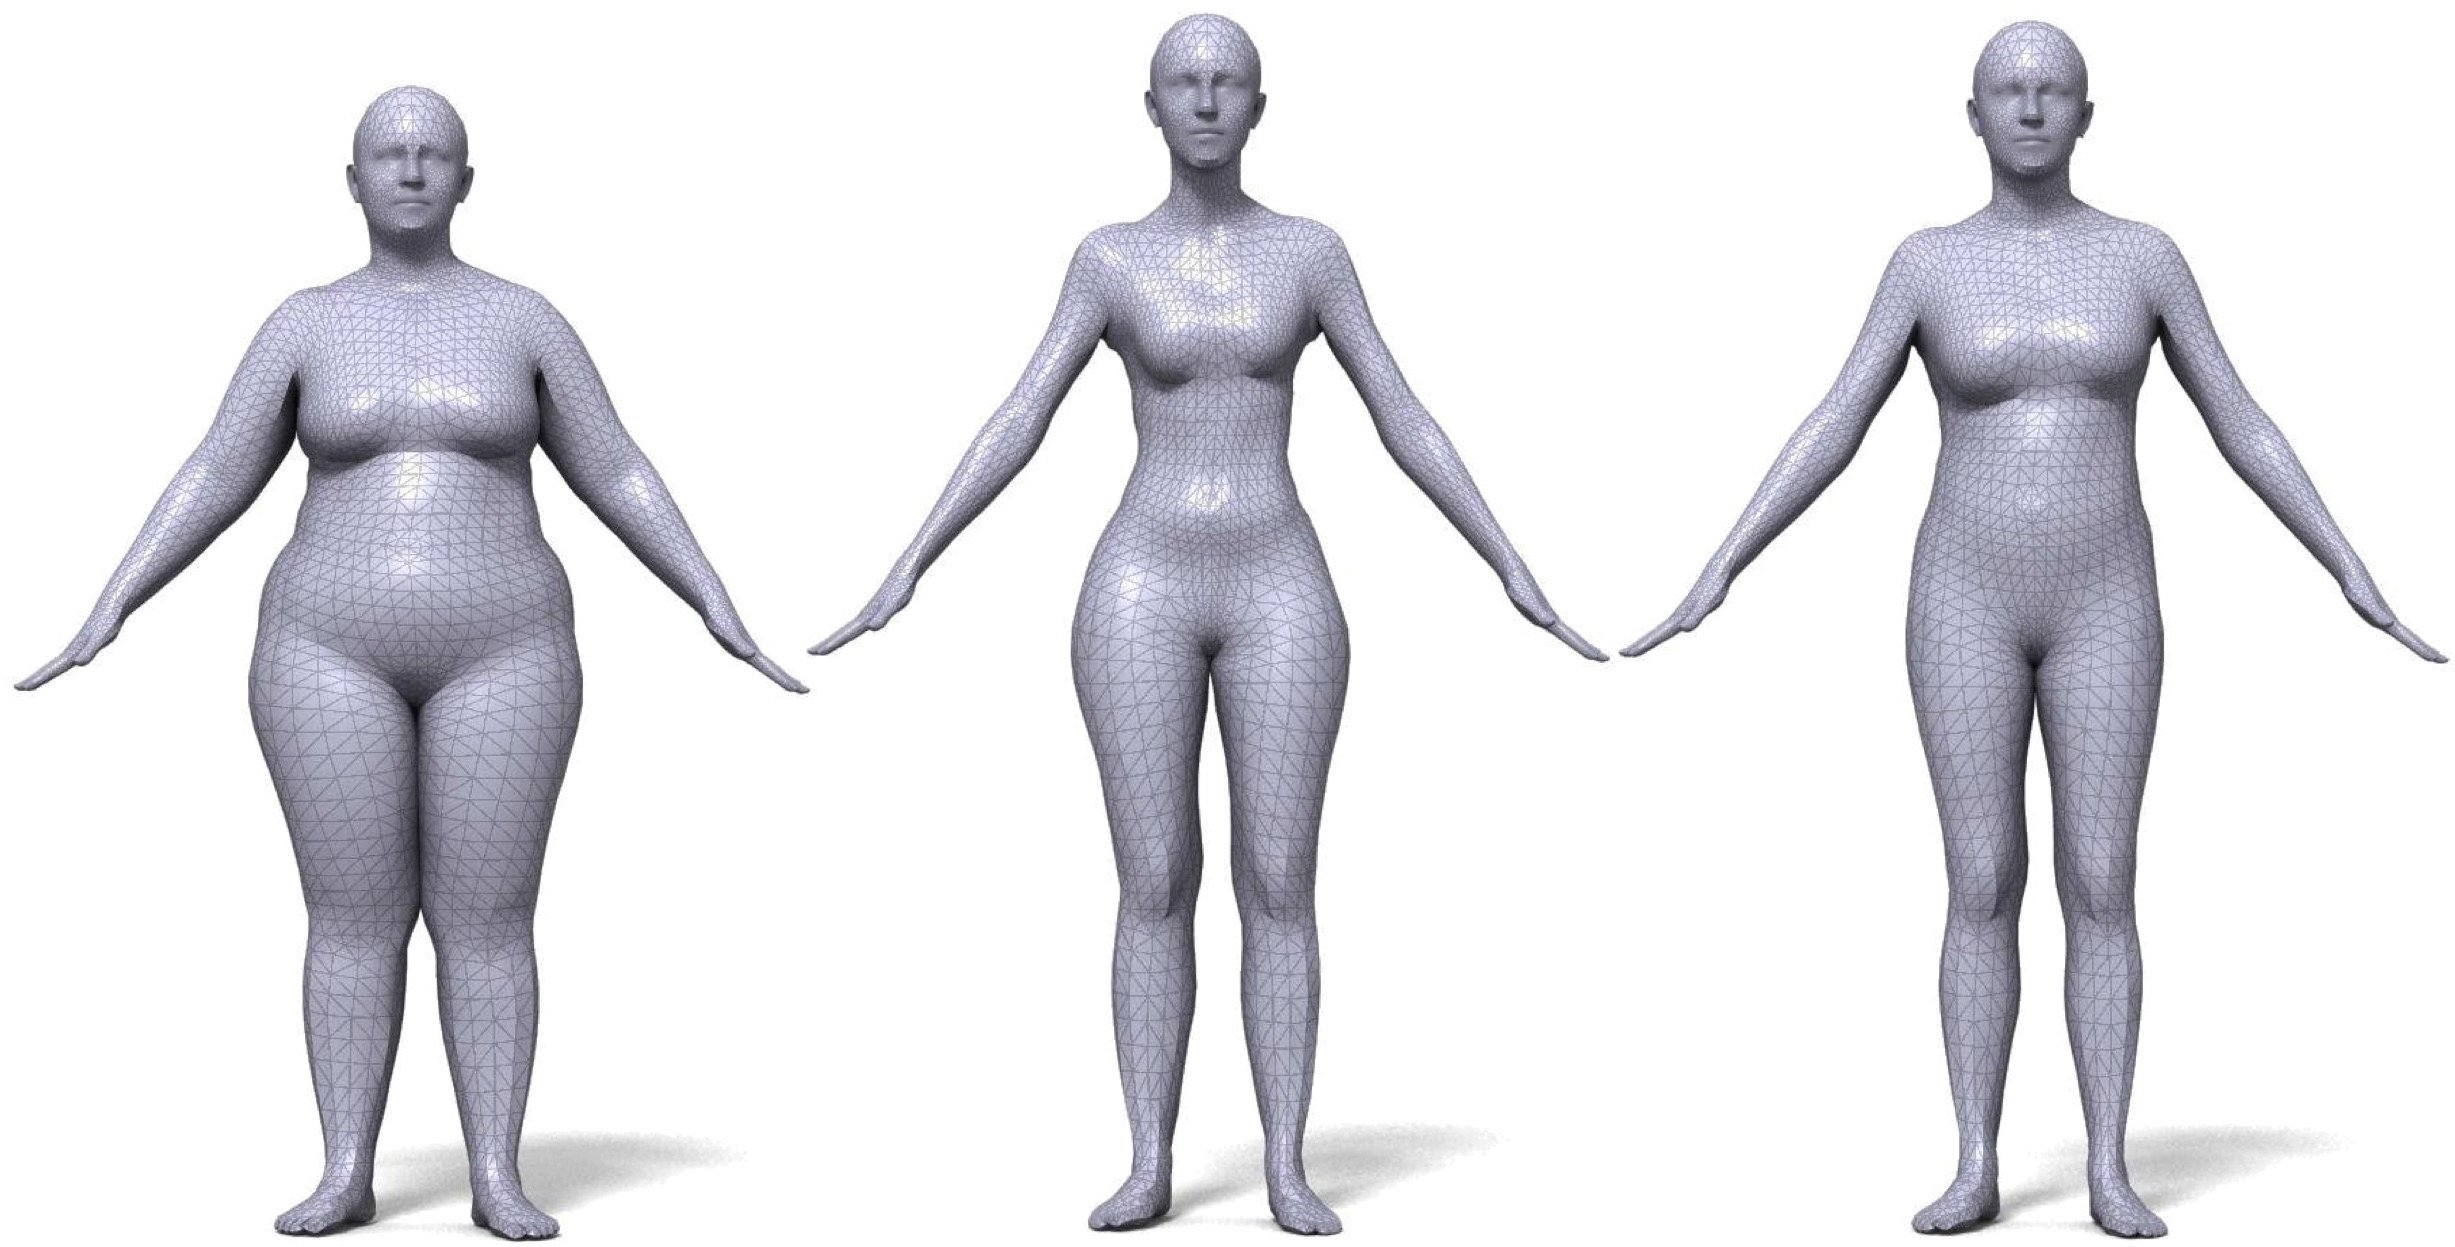
\includegraphics[width=0.9\linewidth]{body_shapes}}
        \caption{Varying human shape parameters while pose remains fixed. Reprinted from~\cite{Streuber:SIGGRAPH:2016}.}
        \label{fig:black_shape}
    \end{figure}
    
    Shape and pose parameters derived from a video sequence can be applied to the template mesh to generate a digital version of the same activity. If successful, the changing parameters should appear to adapt (or morph) the template mesh to faithfully reconstruct the performance given by the original live animal. In early experimentation, in which tracking targets are restricted to the same species, the template can be chosen to be a close shape fit to the target animal, thereby largely reducing the problem to finding optimal per-frame pose parameters. However, tracking examples are eventually broadened to include a wide range of animal species.

    \subsection{Relation to human reconstruction}
    % NEEDS TIDYING
    Given that human tracking is now an established computer vision subfield, and the growing interest in analysing human behaviour from CCTV camera tracking systems, it is natural to ask whether the techniques used in this work transfer to the animal case. As an emerging research field, animal tracking presents many challenges in common with human gait and pose tracking problems, particularly in accurately monitoring morphable objects which frequently self-occlude. However, notable additional challenges are posed by the large shape and texture variation between animal tracking candidates and also due to the lack of available training data which could otherwise be employed to train deep neural networks. An advantageous aspect of tracking animals over humans is the simple fact that animals tend not to wear clothing, which in humans causes significant shape and appearance variability.

    The previous chapter discussed the primary objective of this work, which is to recover full 3D shape and pose from a live input video sequence exhibiting an animal subject. As explained, the major challenge common to all methods operating on monocular RGB input is to resolve the inherent depth ambiguity associated with recovering a 3D model from 2D input. Competitive methods achieve this by relying on strong motion cues~\cite{kinect_fusion} or (if available) by incorporating strong prior knowledge of the tracking target. Strong shape and pose priors (e.g. body part configuration, acceptable body part lengths, likely joint positions etc.) are available for this problem, so this report will focus on analysing these methods in the literature.

    All solutions face an important design decision, which is to make a distinction between features of an input sequence the system should aim to model and to which it should remain invariant. For example, nearly all human systems aim to model the angle between a tracking target's upper and lower leg region, but nearly all will attempt to remain invariant to skin colour variation between candidates. The next two sections discuss examples of systems in which this decision has been made differently, generally according to the intended real-world application.

    We address this problem using techniques from the recent human body and hand tracking literature, combining machine learning and 3D model fitting.  A discriminative front-end uses a deep hourglass network to identify candidate 2D joint positions. These joint positions are then linked into coherent skeletons by solving an optimal joint assignment problem, and the resulting skeletons create an initial estimate for a generative model-fitting back-end to yield detailed shape and pose for each frame of the video.  

    Although superficially similar to human tracking, animal tracking (AT) has some interesting differences that make it worthy of study:

    \subsubsection*{Variability.}
    In one sense, AT is simpler than human tracking as animals generally do not wear clothing. However, variations in surface texture are still considerable between individuals, and the variety of shape across and within species is considerably greater.  If tracking is specialized to a particular species, then shape variation is smaller, but training data is even harder to obtain.

    \subsubsection*{Training data.}
    For human tracking, hand labelled sequences of 2D segmentations and joint positions have been collected from a wide variety of sources~\cite{andriluka14cvpr,lin2014microsoft,johnson2010clustered}. Of these two classes of labelling, animal {\em segmentation} data is available in datasets such as MSCOCO~\cite{lin2014microsoft}, PASCAL VOC~\cite{everingham2010pascal} and DAVIS~\cite{Perazzi2016}.  However this data is considerably sparser than human data, and must be ``shared'' across species, meaning the number of examples for a given animal shape class is considerably fewer than is available for an equivalent variation in human shape.  While segmentation data can be supplied by non-specialist human labellers, it is more difficult to obtain {\em joint position} data.  Some joints are easy to label, such as ``tip of snout'', but others such as the analogue of ``right elbow'' require training of the operator to correctly identify across species.

    Of more concern however, is 3D skeleton data.  For humans, motion capture (mocap) can be used to obtain long sequences of skeleton parameters (joint positions and angles) from a wide variety of motions and activities.
    For animal tracking, this is considerably harder: animals behave differently on treadmills than in their quotidian environments, and although some animals such as horses and dogs have been coaxed into motion capture studios~\cite{wilhelm2015furyexplorer}, it remains impractical to consider mocap for a family of tigers at play.

% \begin{figure}[H] % Example image
%     \center{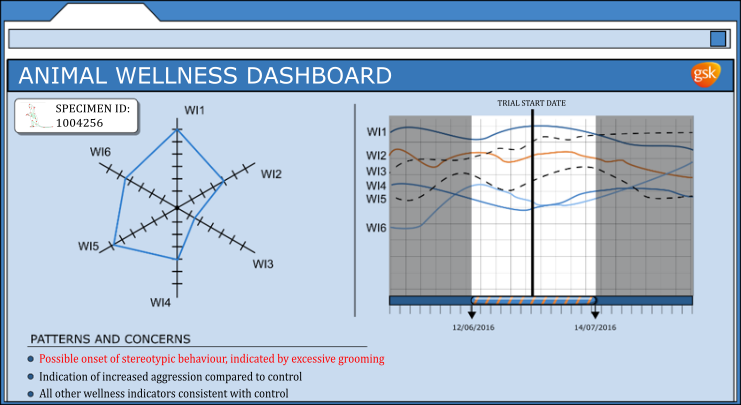
\includegraphics[width=0.95\linewidth]{dash}}
%     \caption{Concept drawing showing an animal health dashboard. Specific wellness markers WI1,...,WI6 have yet to be determined.}
%     \label{fig:wellness_dashboard}
% \end{figure}


%********************************** % Third Section  *************************************
\section{Contributions}  %Section - 1.3 
In summary, the contributions of this thesis are as follows:
\begin{enumerate}
    \item We demonstrate a robust framework for 3D animal reconstruction using deformable template models
\end{enumerate}

\section{Co-Authored Papers}  %Section - 1.4

Extracts from this thesis appear in the following co-authored publications and preprints. \Cref{chap:cgas} contains work from:

\begin{quote}
    \textbf{Benjamin Biggs}, Thomas Roddick, Andrew Fitzgibbon and Roberto Cipolla. \emph{Creatures Great and SMAL: Recovering the Shape and Motion of Animals from Video}. ACCV 2018, Oral Presentation.
\end{quote}

\noindent\Cref{chap:wldo} contains work from:

\begin{quote}
    \textbf{Benjamin Biggs}, Oliver Boyne, James Charles, Andrew Fitzgibbon and Roberto Cipolla. \emph{Who Left the Dogs Out? 3D Animal Reconstruction with Expectation Maximization In the Loop}. ECCV 2020.
\end{quote}

\noindent
\Cref{chap:3dmulti} contains work from:

\begin{quote}
    \textbf{Benjamin Biggs}, Sebastien Ehrhadt, Hanbyul Joo, Benjamin Graham, Andrea Vedaldi and David Novotny. \emph{3D Multi-bodies: Fitting Sets of Plausible 3D Human Models to Ambiguous Image Data}. NeurIPS 2020, Spotlight Presentation.
\end{quote}

\section{Thesis Structure}  %Section - 1.3 

The following thesis chapters discuss methods for deriving 3D animal reconstructions from monocular input images and video. \Cref{chap:intro} begins by covering the necessary background and motivation before an in-depth literature review in \Cref{chap:relwork}. \Cref{chap:cgas} discusses an approach for animal reconstruction learning only from synthetic training data. \Cref{chap:wldo} describes an end-to-end and real-time technique applied to the challenging dog category. \Cref{chap:3dmulti} introduces a method for handling input images with significant ambiguity. The final \Cref{chap:summary} summarizes the work and offers a discussion for worthy future endeavours in the field.